
% this file is called up by thesis.tex
% content in this file will be fed into the main document

%: ----------------------- introduction file header -----------------------
\chapter{Large-scale Comparisons of Topic Distributions}\label{ch:comparisons}

\graphicspath{{comparisons/figures/}}

% -------------------------------------------------------------
% -- Comparisons
% -------------------------------------------------------------

As we showed in Section \ref{sec:topic-clustering}, grouping topics by a cumulative ranking is a useful mechanism for simplifying representations based on topic distributions. Relevant topics emerge as those whose accumulated weight exceeds a threshold, after ordering all topics and starting from the top. This technique has shown a promising performance to cluster documents ( Section \ref{sec:clustering-results}) and  suggests that \textit{similar documents share the most relevant topics}. However, the approach still has limitations: it depends on the manual tuning of a parameter, the threshold; and it does not measure degrees of similarity since it only establishes whether or not two documents are similar. As shown in Chapter \ref{ch:hypothesis}, we hypothesize that is possible to find relevant documents with similar topic distributions without calculating all pairwise comparisons and without discarding the notion of topics from their representation. In this chapter we introduce relevance levels between topics and present our approach to compare documents from huge collections through hierarchical representations of their topic distributions \citep{Badenes-Olmedo2019}.

\section{Hashing Topic Distributions}
\label{sec:comparison-hashing}

One of the greatest advantages of using Probabilistic Topic Models (PTM) in large document collections is the ability to represent documents as probability distributions over a small number of topics, thereby mapping documents into a low-dimensional latent space (the K-dimensional probability simplex, where K is the number of topics). A document, represented as a point in this simplex, is said to have a particular topic distribution. As seen in Section \ref{sec:topic-clustering}, the low-dimensional feature space created by topic models could also be suitable for document similarity tasks, especially on big real-world data sets, since topic distributions are continuous and not as sparse as discrete-term feature vectors and can be explained in terms of relevance. 

Hashing methods transform the data points from the original feature space into a binary-code Hamming space, where the similarities in the original space are preserved. They can learn hash functions (data-dependent) or use projections (data-independent) from the training data \cite{Wang2016}. Data-independent methods unlike data-dependent ones do not need to be re-calculated when data changes, i.e. adding or removing documents to the collection. Taking large-scale scenarios into account (e.g. Document clustering, Content-based Recommendation, Duplicate Detection), this is a key feature along with the ability to infer hash codes individually (for each document) rather than on a set of documents. 

Data-independent hashing methods depend on two key elements: (1) data type and (2) distance metric. For vector-type data, as introduced in Section \ref{sec:related-work}, based on $l_p$ distance with $p \epsilon [0,2)$ lots of hashing methods have been proposed, such as p-stable Locality-Sensitive Hashing (LSH) \citep{Datar2004}, Leech lattice LSH \citep{Andoni2006}, Spherical LSH \citep{Terasawa2007}, and Beyond LSH \citep{Andoni2014}. Based on the $\theta$ distance many methods have been developed such as Kernel LSH \citep{Kulis2012} and Hyperplane hashing \citep{Vijayanarasimhan2014}. But only few methods handle density metrics in a simplex space. A first approach transformed the $He$ divergence into an Euclidean distance so that existing ANN techniques, such as LSH and k-d tree, could be applied \citep{Krstovski2013a}. But this solution does not consider the special attributions of probability distributions, such as Non-negative and Sum-equal-one. Recently, a hashing schema \citep{Mao2017} taking into account the symmetry has been proposed, non-negativity and triangle inequality features of the S2JSD metric for probability distributions. For set-type data, Jaccard Coefficient is the main metric used. Some examples are K-min Sketch \citep{Li2012}, Min-max hash \citep{Ji2013}, B-bit minwise hashing \citep{Li2010b} and Sim-min-hash \citep{Zhao2013}.

All of them have demonstrated efficiency in the search for similar documents, but none of them allows the search for documents (1) by thematic areas or (2) by similarity levels, nor they offer (3) an explanation about the similarity obtained beyond the vectors used to calculate it. Binary-hash codes drop a very precious information: the topic relevance.

A new hierarchical set-type data is proposed (Figure \ref{fig:hash_functions}). Each level of the hierarchy indicates the importance of the topic according to its distribution. Level 0 contains the topics with the highest score. Level 1 contains the topics with highest score once the first ones have been eliminated, and so on. From a vector of components, where each of the components is the score of topic $t$, a  vector containing set of topics is proposed, where each of the dimensions means a topic relevance. Thus, for the topic distribution
$q=[0.02,0.14,0.02,0.16,0.04,0.09,0.19,0.12,0.04,0.17]$, a hierarchical set of topics may be $h=\left \{(t6),(t9,t3),(t1) \right \}$. It means that topic $t6$ (0.19) is the most relevant, then topics $t9$ (0.17) and $t3$ (0.16) and, finally, topic $t1$ (0.14). This is just an example about the data structure that will support the different hashing strategies. In Section \ref{sec:comparison-hash} some approaches to create hash codes based on this data structure are described.

\begin{figure*}
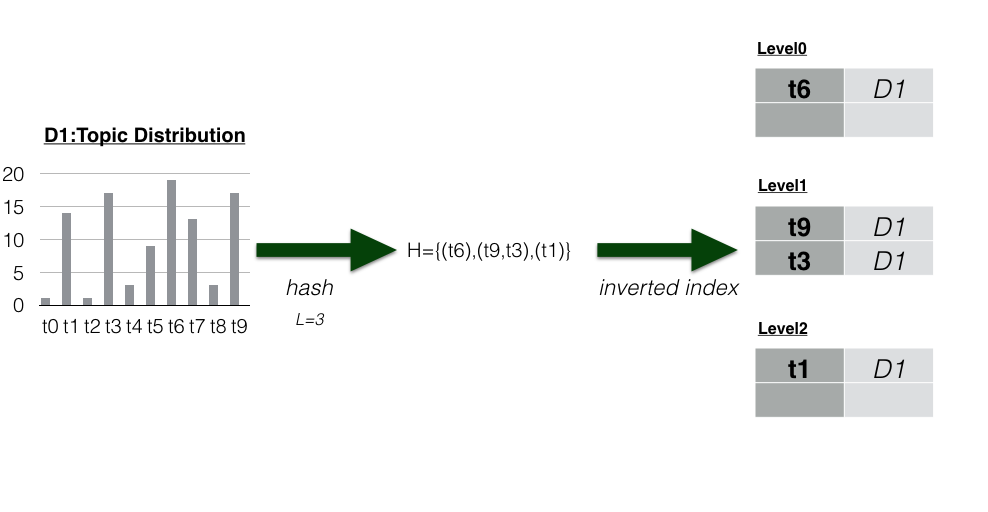
\includegraphics[width=\textwidth,height=9cm]{hashFunctions.png}
\caption{Hash method based on hierarchical set of topics from a given topic distribution}
\label{fig:hash_functions}
\end{figure*}

\subsection{Data Type}
\label{sec:comparison-datatype}
As seen in Section \ref{sec:related-work}, a traditional approach to text representation usually requires encoding of documents into numerical vectors. Words are extracted from a corpus as feature candidates and based on a certain criterion they are assigned values to describe the documents: term-frequency, TF-IDF, information gain, and chi-square are typical measures. But this causes two main problems: huge number of dimensions and sparse distribution. The use of topics as feature space has been extended to mapping documents into low-dimensional vectors. However, as shown in Figure \ref{fig:topic_distances}, the distance metrics based on probability densities vary according to the dimensions of the model and reveal the difficulty of calculating the similarity values using the vectors with the topic distributions.  

Since hashing techniques can transform both vector and set-based data \citep{Mao2017, Ji2013} into a new space where the similarity (i.e. closeness of points) in the original feature space is preserved, a new set-based data structure is proposed in this paper. It is created from clusters of topics organized by relevance levels and it aims to extend the ability of building queries with topic-based restrictions over the searching space while maintaining high level of accuracy.

The new hierarchical set-type data describes each document as a sequence of sets of topics sorted by relevance. Each level of the hierarchy expresses how important those topics are in that document. In the first level (i.e level 0) are the topics with the highest score. In the second level (i.e level 1) are the topics with the highest score once the first ones have been removed, and so on. In this work, several clustering approaches have been considered to assign topics to each level.

In a feature space created from a PTM with eight topics, for example, each data point $p$ is described by a eight-dimensional vector with the topic distributions: $vp=[t0,t1,t2,t3,t4,t5,t6,t7]$ . Then, given a point $q1=[0.18, 0.15, 0.2, 0.05, 0.14, 0.11, 0.09, 0.08]$, the three-level hierarchical set of topics may be $h=[\{t2\},\{t0\},\{t1,t4\}]$. It means that $t2$ is the most relevant topic, then topic $t0$ and finally topics $t1$ and $t4$. This is just an example about the data structure that will support the hashing strategies. In section \ref{sec:comparison-hash} some approaches to create hash codes based on this data structure are described.

Domain-specific features such as vocabulary, writing style, or speech type, have a major influence on the topic models, but not in the hashing algorithms described in this article. The methods for creating hash codes are agnostic of these particularities since they are only based on the topic distributions generated by the models. 

\subsection{Distance Metric}
Since documents are described by set-type data, the proposed distance metric is based on the Jaccard coefficient. This metric computes the similarity of sets by looking at the relative size of their intersection as follows:

%Jaccard Coefficient formula
\begin{equation}
J(A,B) = \frac{ | A \cap B |}{ | A \cup B |}
\label{eq:jc}
\end{equation}
where A and B are set of topics. 

More specifically, $d_J$ is based on the Jaccard distance, which is obtained by subtracting the Jaccard coefficient $J$ from 1:
%Jaccard distance formula
\begin{equation}
d_J(A,B) = 1 - J(A,B)
\label{eq:dj}
\end{equation}

The proposed distance measure $d_H$ used to compare hash codes created from set of topics is the sum of the Jaccard distances $d_j$ for each hierarchy level, i.e. for each set of topics:

%distance metric formula
\begin{equation}
d_H(H_1,H_2) = \sum\limits_{l=1}^L \Big( d_J(H_1(x_l),H_2(x_l)) \Big)
\label{eq:dh}
\end{equation}

where $H_1$ and $H_2$ are hash codes, $H_1(x_l)$ and $H_2(x_l)$ are the set of topics up to level $l$ for each hash code $H$ and $L$ is the maximum hierarchy level. A corner case is $L=T$, where $T$ is the number of topics in the model. 


\subsection{Hash Function}
\label{sec:comparison-hash}

The hash function clusters topics based on relevance levels. Three approaches are proposed depending on the criteria used to group topics: threshold-based, centroid-based and density-based.

\subsubsection{Threshold-based Hierarchical Hashing Method}
\label{sec:comparison-threshold}
This approach is just an initial and naive way of grouping topics by threshold values into each relevance level. They can be manually defined or automatically generated by thresholds dividing the topic distributions as follows:

%threshold formula
\begin{equation}
th_{inc} = \frac{1}{(L+1) \cdot T}
\label{eq:th}
\end{equation}
where $L$ is the number of hierarchy levels, and $T$ the number of topics.

\begin{figure}[t]\centering
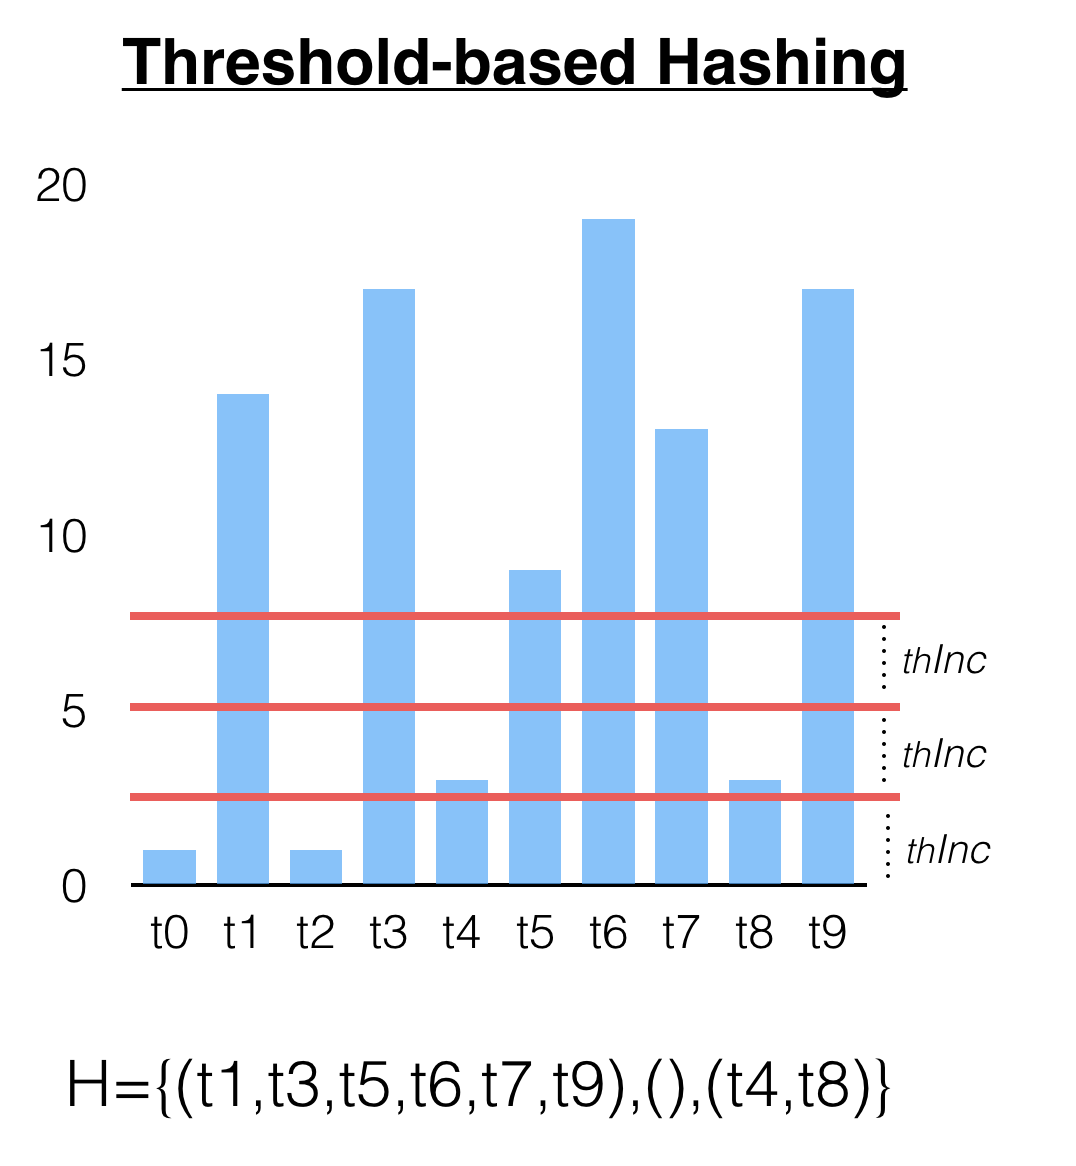
\includegraphics[scale=0.35]{threshold-hash.png}
\caption{Threshold-based Hierarchical Hash (L=3)}
\label{fig:th_hash}
\end{figure}

If $L=3$ and $T=10$ for a topic distribution $td$ defined as follows:
%distance metric formula
\begin{equation}
    \begin{gathered}
td=[0.017, 0.141, 0.010, 0.172, 0.030, \\
0.090, 0.199,  0.133,  0.031, 0.171]
    \end{gathered}
    \label{eq:sample}
\end{equation}

Then, a threshold-based hierarchical hash $H_{T}$, with an automatically created threshold defined by equation \ref{eq:th}, is equals to $H_{T}=\{(t1,t3,t5,t6,t7,t9),(),(t4,t8)\}$ with $th_{inc}=0.025$ (Fig  \ref{fig:th_hash}).

\subsubsection{Centroid-based Hierarchical Hashing Method}
\label{sec:comparison-centroid}
This approach assumes topic distributions can be partitioned into $k$ clusters where each topic belongs to the cluster with the nearest mean score. It is based on the k-Means clustering algorithm, where $k$ is obtained by adding 1 to the number of hierarchy levels. Unlike the previous method, threshold values used to define the hierarchy levels may vary between documents, i.e. for each topic distribution, since they are calculated for each distribution separately.

\begin{figure}[t]\centering
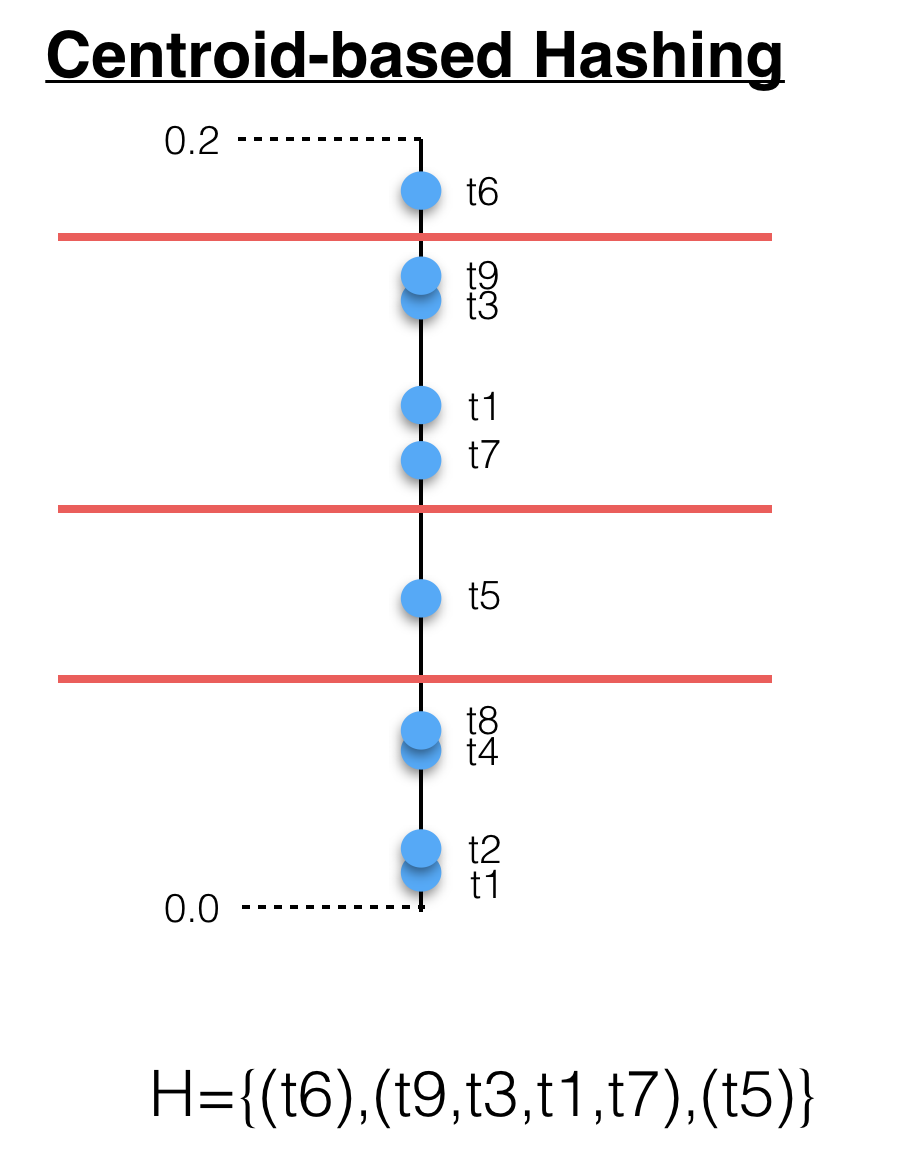
\includegraphics[scale=0.35]{centroid-hash.png}
\caption{Centroid-based Hierarchical Hash (L=3)}
\label{fig:centroid_hash}
\end{figure}

Following the previous example, if $L=3$ and $T=10$ for a topic distribution $td$ defined in equation \ref{eq:sample}, then a centroid-based hieararchical hash $H_{C}$ equals to $H_{C}=\{(t6),(t9,t7,t3,t1),(t5)\}$ (Fig \ref{fig:centroid_hash}).


\subsubsection{Density-based Hierarchical Hashing Method}
\label{sec:comparison-density}
This approach also considers relative hierarchical thresholds for each relevance level. Now, a topic distribution is described by points in a single dimension. In this space, topics closely packed together are grouped together. This approach does not require a fixed number of groups. It only requires a maximum distance ($eps$) to consider two points close and grouped together. This value can be estimated from the own distribution of topics (e.g. variance).

\begin{figure}[t]\centering
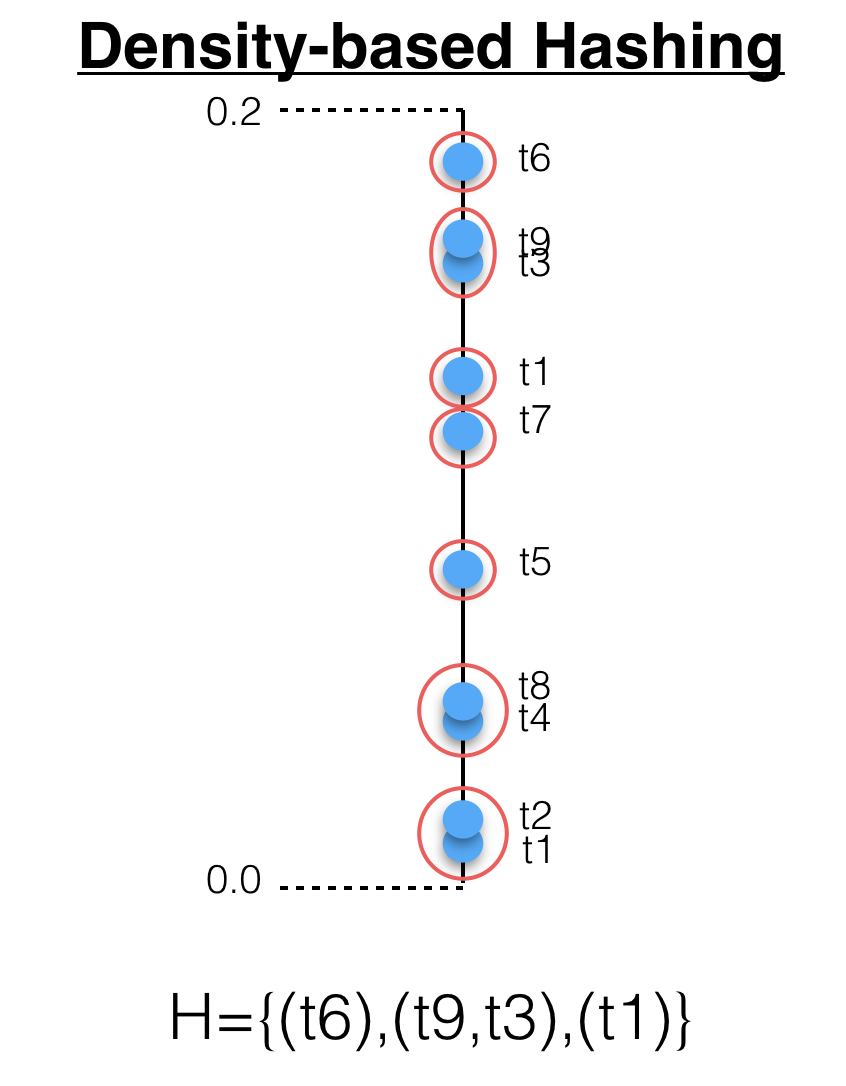
\includegraphics[scale=0.35]{density-hash.png}
\caption{Density-based Hierarchical Hash (L=3)}
\label{fig:density_hash}
\end{figure}

Following the above example, if $L=3$ and $td$ is the topic distribution defined in equation \ref{eq:sample}, then a density-based hierarchical hash $H_{D}$ is equals to $H_{D}=\{(t6),(t9,t3),(t1)\}$ when $eps$ equals to the variance of the topic distribution (Fig \ref{fig:density_hash}).


\subsection{Online-mode Hashing}
\label{sec:comparison-onlineHashing}

Hashing methods are batch-mode learning models that require huge data for learning an optimal model and cannot handle unseen data. Recent work address online mode by learning algorithms \citep{Huang2018} that get hashing model accommodate to each new pair of data. But these approaches require the hashing model to be updated during each round based on the new pairs of data.

Our methods rely on topic models to build hash codes. These models do not require to be updated to make inferences about data not seen during training. In this way, the proposed hashing algorithms can work on large-scale and real-time data, as the size and the novelty of the collection does not influence the annotation process.

\section{Evaluation}
\label{sec:comparison-experiments}

As mentioned in Section \ref{sec:topic-explainability}, it is difficult to interpret the similarity score calculated by metrics in a probability space. Since all of them are based on adding the distance between each dimension of the model (eq. \ref{eq:kl}, \ref{eq:jsdivergence} and \ref{eq:hedistance}), distributions that share a fair amount of the less representative topics may still get higher similarity values than those that share the most representative ones specially if the model has a high number of dimensions.

\begin{figure}[!htb]\centering
   \begin{minipage}{0.49\textwidth}
     \frame{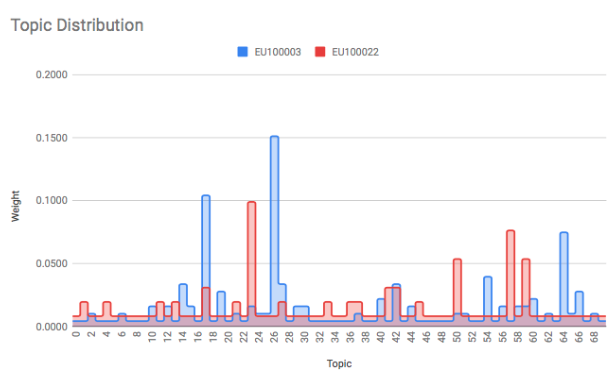
\includegraphics[width=\linewidth]{doc-similarity-pair1.png}}
     \caption{Topic Distribution of two documents with similarity score, based on JSD, equals to 0.74}\label{fig:doc_sim_1}
   \end{minipage}
   \begin {minipage}[c]{0.49\textwidth}
     \frame{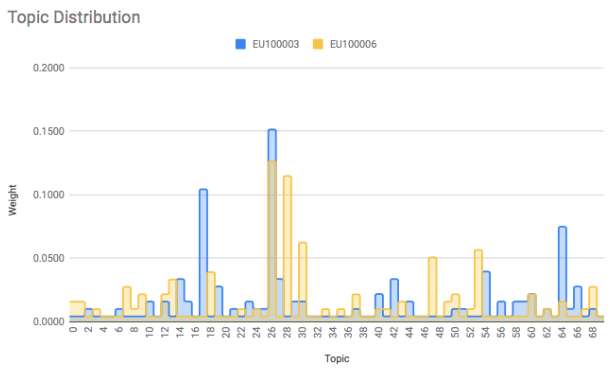
\includegraphics[width=\linewidth]{doc-similarity-pair2.png}}
     \caption{Topic Distribution of two documents with similarity score, based on JSD, equals to 0.71}\label{fig:doc_sim_2}
   \end{minipage}
\end{figure}

Figures \ref{fig:doc_sim_1} and \ref{fig:doc_sim_2} show overlapped topic distributions of two pairs of documents. In the first case (fig  \ref{fig:doc_sim_1}), none of the most representative topics of each document is shared between them. However, the similarity score calculated from divergence-based metrics (eq \ref{eq:jsdivergence}) is higher than in the second case (fig  \ref{fig:doc_sim_2}), where the most representative topic is shared (topic 26). This behavior is due to the sum of the distances between the less representative topics (i.e. topics with a low weight value) being greater than the sum of the distances between the most representative ones (i.e. topic with a high weight value). In high-dimensional models, that sum may be more representative than the one obtained with the most relevant topics, which are fewer in number than the less relevant ones. 

The following experiments aim to validate that \textit{\textbf{hash codes based on hierarchical set of topics not only make it possible to search for similar documents with high accuracy, but also to extend queries with new restrictions and to offer information that helps explaining why two documents are similar}}.

\subsection{Datasets and Evaluation Metrics}
\label{sec:comparison-datasets}
Three datasets \citep{Badenes-Olmedo2019a} are used to validate the proposed approach. The OPEN-RESEARCH\footnote{https://labs.semanticscholar.org/corpus/} dataset consist of 500k research papers in Computer Science, Neuroscience, and Biomedical randomly selected from the Open Research Corpus \citep{Waleed2018}. The CORDIS\footnote{https://data.europa.eu/euodp/data/dataset/cordisref-data} dataset contains 100k documents describing research and innovation projects funded by the European Union under a framework programme since 1990. The PATENTS dataset consists of 1M patents randomly selected from the USPTO\footnote{https://www.uspto.gov/learning-and-resources/ip-policy/economic-research/research-datasets} collection. For each dataset, documents are mapped to two latent topic spaces with different dimensions using LDA. We perform parameter estimation using collapsed Gibbs sampling for LDA \citep{Griffiths2004b} from our librAIry  framework. The number of topics varies to study their influence on the performance of the algorithm (i.e. CORDIS-70 indicates a latent space created with 70 topics). 

Experiments use JS divergence as an information-theoretically motivated metric in the probabilistic space created by topic models. Since it is a smoothed and symmetric alternative to the KL divergence, which is a standard measure for comparing distributions \citep{Cha2007}, it has been extensively used as state-of-the-art metric over topic distributions in literature \citep{Towne2016, Aletras2017, Mao2017}. Our upper bound is created from the brute-force comparison of the reference documents with all documents in the collection to obtain the list of similar documents.  

In this scenario the goal is to minimize the accuracy loss introduced by hashing algorithms. Since this is a large-scale problem and an accuracy-oriented task, recall is not a good measure to be considered and precision is only relevant for sets much smaller than the total size of data (between 3-5 candidates).

All the experimental results are averaged over random training/set partitions. For each topic space, 100 documents are selected as references, and the remaining documents as search space. As noted above, only p@5 will be used to report the results of the experiments.

\subsection{Retrieving Similar Documents}
\label{sec:comparison-search}

It is challenging to create an exhaustive gold standard, given the significant amount of human labour that is required to get a comprehensive view of the subjects being covered in it. In order to overcome this problem, the list of similar documents to a given one is obtained after comparing the document with all the documents of the repository and sorting the result. We have observed that different distance functions perform similarly in this scenario (Fig. \ref{fig:topic_distances}), so we have decided to use only the JS divergence (eq. \ref{eq:jsdivergence}) in our experiments.

Only the top N documents obtained from this method are used as reference set to measure the performance of the algorithms proposed in this paper. The value of N is equals to 0.5\% of the corpus size (i.e. if the corpus size is equal to 1000 elements, only the top 5 most similar documents are considered relevant for a given document). This value has been considered after reviewing datasets used in similar experiments \citep{Krstovski2013a, Mao2017}. In those experiments, the reference data is obtained from existing categories, and the minimum average between corpus size and categorized documents is around 0.5\%. 

Once the reference list of documents similar to a given one is defined, the most similar documents through the proposed methods (i.e. threshold-based hierarchical hashing method (thhm), centroid-based hierarchical hashing method (chhm) and density-based hierarchical hashing method (dhhm)) are also obtained. An inverted index has been implemented by using Apache Lucene\footnote{http://lucene.apache.org} as document repository. The source code of both the algorithms and tests is publicly available \citep{Badenes-Olmedo2019a}. 

\begin{table}\centering
  \scriptsize
  \begin{tabular}{c|rr||rr||rr}
    \multicolumn{7}{c}{OPEN-RES-100 (p@5)} \\
    \toprule
    \multirow{2}{*}{LEVEL} &
      \multicolumn{2}{c}{THHM} &
      \multicolumn{2}{c}{CHHM} &
      \multicolumn{2}{c}{DHHM} \\
      & {\textit{mean}} & {\textit{median}} & {\textit{mean}} & {\textit{median}} & {\textit{mean}} & {\textit{median}} \\
      \midrule
    2 & 0.22 & 0.20 & \textbf{0.86} & 1.00 & 0.66 & 0.80 \\
    3 & 0.23 & 0.20 & \textbf{0.87} & 1.00 & 0.81 & 1.00 \\
    4 & 0.27 & 0.20 & \textbf{0.89} & 1.00 & 0.86 & 1.00 \\
    5 & 0.27 & 0.20 & \textbf{0.92} & 1.00 & 0.89 & 1.00 \\
    6 & 0.27 & 0.20 & \textbf{0.94} & 1.00 & 0.92 & 1.00 \\
    \bottomrule
  \end{tabular}
\caption{Precision at 5 (\textit{mean} and \textit{median}) of threshold-based (THHM), centroid-based (CHHM) and density-based (DHHM) hierarchical hashing methods on Open Research dataset using a model with 100 topics. LEVEL column indicates the number of hierarchies used.}
\label{tb:or100-p}
\end{table}

\begin{table}\centering
  \scriptsize
  \begin{tabular}{c|rr||rr||rr}
    \multicolumn{7}{c}{OPEN-RES-500 (p@5)} \\
    \toprule
    \multirow{2}{*}{LEVEL} &
      \multicolumn{2}{c}{THHM} &
      \multicolumn{2}{c}{CHHM} &
      \multicolumn{2}{c}{DHHM} \\
      & {\textit{mean}} & {\textit{median}} & {\textit{mean}} & {\textit{median}} & {\textit{mean}} & {\textit{median}} \\
      \midrule
    2 & 0.23 & 0.20 & \textbf{0.76} & 0.80 & 0.67 & 0.80 \\
    3 & 0.24 & 0.20 & \textbf{0.80} & 1.00 & 0.71 & 0.80 \\
    4 & 0.25 & 0.20 & \textbf{0.83} & 1.00 & 0.74 & 0.80 \\
    5 & 0.25 & 0.20 & \textbf{0.86} & 1.00 & 0.81 & 1.00 \\
    6 & 0.24 & 0.20 & \textbf{0.89} & 1.00 & 0.86 & 1.00 \\
    \bottomrule
  \end{tabular}
\caption{Precision at 5 (\textit{mean} and \textit{median}) of threshold-based (THHM), centroid-based (CHHM) and density-based (DHHM) hierarchical hashing methods on Open Research dataset using a model with 500 topics. LEVEL column indicates the number of hierarchies used.}
\label{tb:or500-p}
\end{table}

\begin{table}\centering
  \scriptsize
  \begin{tabular}{c|rr||rr||rr}
    \multicolumn{7}{c}{CORDIS-70 (p@5)} \\
    \toprule
    \multirow{2}{*}{LEVEL} &
      \multicolumn{2}{c}{THHM} &
      \multicolumn{2}{c}{CHHM} &
      \multicolumn{2}{c}{DHHM} \\
      & {\textit{mean}} & {\textit{median}} & {\textit{mean}} & {\textit{median}} & {\textit{mean}} & {\textit{median}} \\
      \midrule
    2 & 0.18 & 0.20 & \textbf{0.92} & 1.00 & 0.66 & 0.70 \\
    3 & 0.20 & 0.20 & \textbf{0.92} & 1.00 & 0.80 & 0.80 \\
    4 & 0.22 & 0.20 & \textbf{0.94} & 1.00 & 0.86 & 1.00 \\
    5 & 0.23 & 0.20 & \textbf{0.91} & 1.00 & 0.89 & 1.00 \\
    6 & 0.19 & 0.20 & \textbf{0.92} & 1.00 & 0.91 & 1.00 \\
    \bottomrule
  \end{tabular}
\caption{Precision at 5 (\textit{mean} and \textit{median}) of threshold-based (THHM), centroid-based (CHHM) and density-based (DHHM) hierarchical hashing methods on CORDIS dataset using a model with 70 topics. LEVEL column indicates the number of hierarchies used.}
\label{tb:cordis70-p}
\end{table}


\begin{table}\centering
  \scriptsize
  \begin{tabular}{c|rr||rr||rr}
    \multicolumn{7}{c}{CORDIS-150 (p@5)} \\
    \toprule
    \multirow{2}{*}{LEVEL} &
      \multicolumn{2}{c}{THHM} &
      \multicolumn{2}{c}{CHHM} &
      \multicolumn{2}{c}{DHHM} \\
      & {\textit{mean}} & {\textit{median}} & {\textit{mean}} & {\textit{median}} & {\textit{mean}} & {\textit{median}} \\
      \midrule
     2 & 0.19 & 0.20 & \textbf{0.88} & 1.00 & 0.78 & 0.80 \\
     3 & 0.19 & 0.20 & \textbf{0.92} & 1.00 & 0.80 & 1.00 \\
     4 & 0.25 & 0.20 & \textbf{0.91} & 1.00 & 0.82 & 1.00 \\
     5 & 0.25 & 0.20 & \textbf{0.91} & 1.00 & 0.83 & 1.00 \\
     6 & 0.27 & 0.20 & \textbf{0.91} & 1.00 & 0.86 & 1.00 \\
    \bottomrule
  \end{tabular}
\caption{Precision at 5 (\textit{mean} and \textit{median}) of threshold-based (THHM), centroid-based (CHHM) and density-based (DHHM) hierarchical hashing methods on CORDIS dataset using a model with 150 topics. LEVEL column indicates the number of hierarchies used.}
\label{tb:cordis150-p}
\end{table}

Let's look at an example to better understand the procedure. We want to measure the accuracy and data size ratio used to identify the top5 similar documents to a new document $d_1$ from a corpus of $1000$ documents . The similarity between $d1$ and all the documents in the corpus is calculated based on JS divergence. The top50 ($0.5\%$) documents with the highest values will be the set of documents considered as similar to $d_1$. As we are going to use an ANN-based approach, we need the hash expressions of all documents to measure similarity. The data structure proposed in this work is a hierarchy of sets of topics, so that the most similar documents are those that share most of the topics at the highest levels of the hierarchy.

The representational model for this example only considers 8 topics, that is, a document is described by a vector with $8$ dimensions where each dimension corresponds to a topic (i.e $[t0, t1, t2, t3, t4, t5, t6, t7]$ ) and its value will be the weight of that topic in the document, for example $d_1=[0.18, 0.15, 0.2, 0.05, 0.14, 0.11, 0.09,\\ 0.08]$. The hierarchy level ($L$) will be equal to $2$, i.e. the hash expression has two hierarchical sets of topics: $h=\{h_0, h_1\}$. 

According to methods described at Section \ref{sec:comparison-hash}, there are 3 ways to create the hierarchical hash codes for documents:
\begin{enumerate}
\item \underline{threshold-based} (\textit{thhm}): $2$ thresholds are defined as described in section \ref{sec:comparison-threshold}, for example $0.15$ and $0.1$ . $h_0$ includes the topics with a weight greater than $0.15$, and $h_1$ the remaining topics with a weight greater than $0.1$. Then $h_0=\{t0,t1,t2\}$ and $h_1=\{t4,t5\}$. Based on the hash expression $h=\{(t0,t1,t2),(t4,t5)\}$, the documents that share more topics in those levels (i.e $h0=(t0$ OR $t1$ OR $t2)$, $h1=(t4$ OR $t5)$) or in other levels but with less relevance are ordered. Since there are many topics in the expression, potentially many documents are similar when sharing at least one of them. This increases the data ratio. Accuracy is also affected, as the algorithm is not able to bring under the same bucket similar documents. In short, the hash expression is not representative of the document, for the given exploratory task.
\item \underline{centroid-based} (\textit{chhm}): sets of topics are created using a clustering algorithm based on centroids as described in section \ref{sec:comparison-centroid}. The cardinalities of the hierarchical groups are generally more uniform with this method. Since $k=L+1=3$ in this example, $h_0=\{t0,t2\}$ and $h_1=\{t1,t4\}$. The number of representative topics at each level of the hierarchy is usually lower, and this causes the data ratio used to discover similar documents to decrease as well. This approach increases the precision because now the hierarchy is more selective to distinguish similar documents. However, the size of region of similar candidates is still high.
\item \underline{density-based} (\textit{dhhm}): now the clustering algorithm is based on how dense certain regions in the topic relevance dimensions are as described in section \ref{sec:comparison-density}. It can group topics that have unbalanced distributions and, therefore, generates more discriminating hash expressions than with the previous algorithm. In the example, we would have a hash expression like this: $h_0=\{t2\}$ and $h_1=\{t0\}$. This significantly reduces the data ratio used to discover similar documents and does not excessively penalize accuracy. Obviously, increasing $L$ (i.e. number of hierarchies) increases precision, but with $L>3$ that gain is not so significant.
\end{enumerate}

\begin{table}\centering
  \scriptsize
  \begin{tabular}{c|rr||rr||rr}
    \multicolumn{7}{c}{PATENTS-250 (p@5)} \\
    \toprule
    \multirow{2}{*}{LEVEL} &
      \multicolumn{2}{c}{THHM} &
      \multicolumn{2}{c}{CHHM} &
      \multicolumn{2}{c}{DHHM} \\
      & {\textit{mean}} & {\textit{median}} & {\textit{mean}} & {\textit{median}} & {\textit{mean}} & {\textit{median}} \\
      \midrule
     2 & 0.03 & 0.00 & \textbf{0.71} & 0.80 & 0.67 & 0.80 \\
     3 & 0.08 & 0.00 & \textbf{0.91} & 1.00 & 0.90 & 1.00 \\
     4 & 0.11 & 0.00 & \textbf{0.95} & 1.00 & \textbf{0.95} & 1.00 \\
     5 & 0.12 & 0.00 & 0.95 & 1.00 & \textbf{0.96} & 1.00 \\
     6 & 0.11 & 0.00 & \textbf{0.97} & 1.00 & \textbf{0.97} & 1.00 \\
    \bottomrule
  \end{tabular}
\caption{Precision at 5 (\textit{mean} and \textit{median}) of threshold-based (THHM), centroid-based (CHHM) and density-based (DHHM) hierarchical hashing methods on Patents dataset using a model with 250 topics. LEVEL column indicates the number of hierarchies used.}
\label{tb:patents250-p}
\end{table}


\begin{table}\centering
  \scriptsize
  \begin{tabular}{c|rr||rr||rr}
    \multicolumn{7}{c}{PATENTS-750 (p@5)} \\
    \toprule
    \multirow{2}{*}{LEVEL} &
      \multicolumn{2}{c}{THHM} &
      \multicolumn{2}{c}{CHHM} &
      \multicolumn{2}{c}{DHHM} \\
      & {\textit{mean}} & {\textit{median}} & {\textit{mean}} & {\textit{median}} & {\textit{mean}} & {\textit{median}} \\
      \midrule
     2 & 0.02 & 0.00 & \textbf{0.77} & 0.80 & 0.76 & 0.80 \\
     3 & 0.04 & 0.00 & 0.94 & 1.00 & \textbf{0.95} & 1.00 \\
     4 & 0.06 & 0.00 & \textbf{0.97} & 1.00 & \textbf{0.97} & 1.00 \\
     5 & 0.08 & 0.00 & \textbf{0.97} & 1.00 & \textbf{0.97} & 1.00 \\
     6 & 0.06 & 0.00 & \textbf{0.97} & 1.00 & \textbf{0.97} & 1.00 \\
    \bottomrule
  \end{tabular}
\caption{Precision at 5 (\textit{mean} and \textit{median}) of threshold-based (THHM), centroid-based (CHHM) and density-based (DHHM) hierarchical hashing methods on Patents dataset using a model with 750 topics. LEVEL column indicates the number of hierarchies used.}
\label{tb:patents750-p}
\end{table}

\begin{table}\centering
  \scriptsize
  \begin{tabular}{c|rr||rr||rr}
    \multicolumn{7}{c}{OPEN-RES-100 (data-ratio)} \\
    \toprule
    \multirow{2}{*}{LEVEL} &
      \multicolumn{2}{c}{THHM} &
      \multicolumn{2}{c}{CHHM} &
      \multicolumn{2}{c}{DHHM} \\
      & {\textit{mean}} & {\textit{median}} & {\textit{mean}} & {\textit{median}} & {\textit{mean}} & {\textit{median}} \\
      \midrule
    2 & 99.8 & 99.9 & 45.2 & 45.9 & \textbf{4.9} & 2.5 \\
    3 & 99.9 & 99.9 & 74.4 & 77.6 & \textbf{13.4} & 10.7 \\
    4 & 99.9 & 99.9 & 87.4 & 90.2 & \textbf{27.2} & 22.8 \\
    5 & 99.9 & 99.9 & 95.4 & 96.3 & \textbf{49.9} & 42.6 \\
    6 & 99.9 & 99.9 & 97.9 & 98.7 & \textbf{72.2} & 65.8 \\
    \bottomrule
  \end{tabular}
\caption{Data size ratio used (\textit{mean} and \textit{median}) of threshold-based (THHM), centroid-based (CHHM) and density-based (DHHM) hierarchical hashing methods on Open Research dataset and 100 topics.}
\label{tb:or100-d}
\end{table}

\begin{table}\centering
  \scriptsize
  \begin{tabular}{c|rr||rr||rr}
    \multicolumn{7}{c}{OPEN-RES-500 (data-ratio)} \\
    \toprule
    \multirow{2}{*}{LEVEL} &
      \multicolumn{2}{c}{THHM} &
      \multicolumn{2}{c}{CHHM} &
      \multicolumn{2}{c}{DHHM} \\
      & {\textit{mean}} & {\textit{median}} & {\textit{mean}} & {\textit{median}} & {\textit{mean}} & {\textit{median}} \\
      \midrule
    2 & 95.9 & 96.3 & 22.2 & 22.1 & \textbf{1.4} & 0.3 \\
    3 & 99.1 & 99.2 & 43.9 & 43.7 & \textbf{5.1} & 4.1 \\
    4 & 99.6 & 99.6 & 57.1 & 57.3 & \textbf{11.7} & 10.3 \\
    5 & 99.6 & 99.6 & 70.7 & 70.7 & \textbf{28.8} & 22.0 \\
    6 & 99.9 & 99.9 & 81.5 & 80.6 & \textbf{50.3} & 40.1 \\
    \bottomrule
  \end{tabular}
\caption{Data size ratio used (\textit{mean} and \textit{median}) of threshold-based (THHM), centroid-based (CHHM) and density-based (DHHM) hierarchical hashing methods on Open Research dataset and 500 topics.}
\label{tb:or500-d}
\end{table}

As it can be seen in tables \ref{tb:or100-p} to \ref{tb:patents750-p}, the mean and median of precision are calculated to compare the performance of the methods. In this assessment environment, the variance is not robust-enough because score values don't follow a normal distribution. We consider the result obtained as significant, based on the fact that mean and median values are fairly close. The centroid-based method (chhm) and the density-based method (dhhm) show a similar behaviour to the one offered by the use of brute force by means of JS divergence. 

In terms of efficiency, we consider the times to compare pairs of topic distributions constant, and we focus on the number of comparisons needed. Thus, algorithms with larger candidate spaces will be less efficient than others when the accuracy in both is the same. Tables \ref{tb:or100-d}-\ref{tb:patents750-d} show the percentage of the corpus used by each of the algorithms to discover similar documents. Tables \ref{tb:or100-p}-\ref{tb:patents750-p} show the accuracy of each algorithm for each of these scenarios. Density-based algorithm (dhhm) shows better balance between accuracy and volume of information (efficiency). It uses smaller samples (i.e lower ratio size) than others in all tests and even when it only uses a subset that is a $6.2\%$ (Table \ref{tb:cordis150-d}) of the entire corpus, it obtains an accuracy of $0.808$ (Table \ref{tb:cordis150-p}).


\begin{table}\centering
  \scriptsize
  \begin{tabular}{c|rr||rr||rr}
    \multicolumn{7}{c}{CORDIS-70 (data-ratio)} \\
    \toprule
    \multirow{2}{*}{LEVEL} &
      \multicolumn{2}{c}{THHM} &
      \multicolumn{2}{c}{CHHM} &
      \multicolumn{2}{c}{DHHM} \\
      & {\textit{mean}} & {\textit{median}} & {\textit{mean}} & {\textit{median}} & {\textit{mean}} & {\textit{median}} \\
      \midrule
    2 & 99.9 & 99.9 & 51.3 & 56.3 & \textbf{5.1} & 5.0 \\
    3 & 99.9 & 99.9 & 84.8 & 89.5 & \textbf{10.5} & 10.6 \\
    4 & 99.9 & 99.9 & 96.1 & 97.6 & \textbf{20.8} & 19.5 \\
    5 & 99.9 & 99.9 & 98.9 & 99.4 & \textbf{35.0} & 32.7 \\
    6 & 99.9 & 99.9 & 99.7 & 99.8 & \textbf{53.1} & 51.2 \\
    \bottomrule
  \end{tabular}
\caption{Data size ratio used (\textit{mean} and \textit{median}) of threshold-based (THHM), centroid-based (CHHM) and density-based (DHHM) hierarchical hashing methods on CORDIS dataset and 70 topics.}
\label{tb:cordis70-d}
\end{table}

\begin{table}\centering
  \scriptsize
  \begin{tabular}{c|rr||rr||rr}
    \multicolumn{7}{c}{CORDIS-150 (data-ratio)} \\
    \toprule
    \multirow{2}{*}{LEVEL} &
      \multicolumn{2}{c}{THHM} &
      \multicolumn{2}{c}{CHHM} &
      \multicolumn{2}{c}{DHHM} \\
      & {\textit{mean}} & {\textit{median}} & {\textit{mean}} & {\textit{median}} & {\textit{mean}} & {\textit{median}} \\
      \midrule
    2 & 99.9 & 99.9 & 40.9 & 41.2 & \textbf{3.1} & 2.9 \\
    3 & 99.9 & 99.9 & 75.3 & 76.7 & \textbf{6.2} & 6.1 \\
    4 & 99.9 & 99.9 & 90.0 & 92.1 & \textbf{12.1} & 11.8 \\
    5 & 99.9 & 99.9 & 96.4 & 96.9 & \textbf{21.6} & 20.6 \\
    6 & 99.9 & 99.9 & 98.1 & 98.9 & \textbf{36.5} & 33.9 \\
    \bottomrule
  \end{tabular}
\caption{Data size ratio used (\textit{mean} and \textit{median}) of threshold-based (THHM), centroid-based (CHHM) and density-based (DHHM) hierarchical hashing methods on CORDIS dataset and 150 topics.}
\label{tb:cordis150-d}
\end{table}

The precision achieved by the algorithm based on density (dhhm), which is much more restrictive than the others, suggests that few topics are required to represent a document in order to obtain similar ones. In addition, the number of topics does not seem to influence the performance of the algorithms, since their precision values are similar among the datasets of the same corpus. This shows that hashing methods based on hierarchical set of topics are robust to models with different dimensions.


\begin{table}\centering
  \scriptsize
  \begin{tabular}{c|rr||rr||rr}
    \multicolumn{7}{c}{PATENTS-250 (data-ratio)} \\
    \toprule
    \multirow{2}{*}{LEVEL} &
      \multicolumn{2}{c}{THHM} &
      \multicolumn{2}{c}{CHHM} &
      \multicolumn{2}{c}{DHHM} \\
      & {\textit{mean}} & {\textit{median}} & {\textit{mean}} & {\textit{median}} & {\textit{mean}} & {\textit{median}} \\
      \midrule
    2 & 99.9 & 99.9   & 43.2 & 32.7  & \textbf{35.1} & 23.0 \\
    3 & 99.9 & 100.0  & 82.4 & 100.0 & \textbf{78.2} & 100.0 \\
    4 & 99.9 & 100.0  & 96.5 & 100.0 & \textbf{95.1} & 100.0 \\
    5 & 99.9 & 99.9   & 99.2 & 100.0 & \textbf{98.9} & 100.0 \\
    6 & 100.0 & 100.0 & 99.8 & 100.0 & \textbf{99.7} & 100.0 \\
    \bottomrule
  \end{tabular}
\caption{Data size ratio used (\textit{mean} and \textit{median}) of threshold-based (THHM), centroid-based (CHHM) and density-based (DHHM) hierarchical hashing methods on Patents dataset and 250 topics.}
\label{tb:patents250-d}
\end{table}

\begin{table}\centering
  \scriptsize
  \begin{tabular}{c|rr||rr||rr}
    \multicolumn{7}{c}{PATENTS-750 (data-ratio)} \\
    \toprule
    \multirow{2}{*}{LEVEL} &
      \multicolumn{2}{c}{THHM} &
      \multicolumn{2}{c}{CHHM} &
      \multicolumn{2}{c}{DHHM} \\
      & {\textit{mean}} & {\textit{median}} & {\textit{mean}} & {\textit{median}} & {\textit{mean}} & {\textit{median}} \\
      \midrule
    2 & 99.9 & 100.0 & 35.2 & 23.6 & \textbf{31.8} & 19.9 \\
    3 & 99.9 & 99.9  & 81.4 & 99.8 & \textbf{79.6} & 98.8 \\
    4 & 99.9 & 99.9  & 96.5 & 99.9 & \textbf{95.5} & 99.5 \\
    5 & 97.7 & 96.6  & 99.0 & 99.9 & \textbf{98.6} & 99.7 \\
    6 & 99.1 & 98.6  & 99.7 & 99.9 & \textbf{99.5} & 99.8 \\
    \bottomrule
  \end{tabular}
\caption{Data size ratio used (\textit{mean} and \textit{median}) of threshold-based (THHM), centroid-based (CHHM) and density-based (DHHM) hierarchical hashing methods on Patents dataset and 750 topics.}
\label{tb:patents750-d}
\end{table}

The behavior of the algorithms have also been analyzed when the number of topics in the model varies. Models with 100, 200, 300, 400, 500, 600, 700, 800, 900 and 1000 topics were created from the CORDIS corpus. For each model, the p@5 of the hashing methods is calculated taking into account the hierarchy levels: 2, 3, 4, 5 and 6. Figures \ref{fig:thhm_pd} to \ref{fig:dhhm_pd} show the results obtained for each algorithm. It can be seen how the performance, i.e precision, of each of the algorithms is not influenced by the dimensions of the model.

\subsection{Exploration}
\label{sec:comparison-exploration}

In a certain domain, we may want to retrieve similar documents to one given. For example, searching for articles in the Biomedical domain that are similar to an article about Semantic Web. In terms of topics this kind of search requires to narrow down the initial search space to a subset with only documents that contain the topics that better describe the queried domain.

Existing hashing techniques based on a binary-code Hamming space do not allow to customize the search query beyond the reference document itself. However, the algorithms proposed in this work allow adding new restrictions to the initial query based on the reference document, since they use a hierarchy of set of topics as hash codes.

\begin{figure}[t]\centering
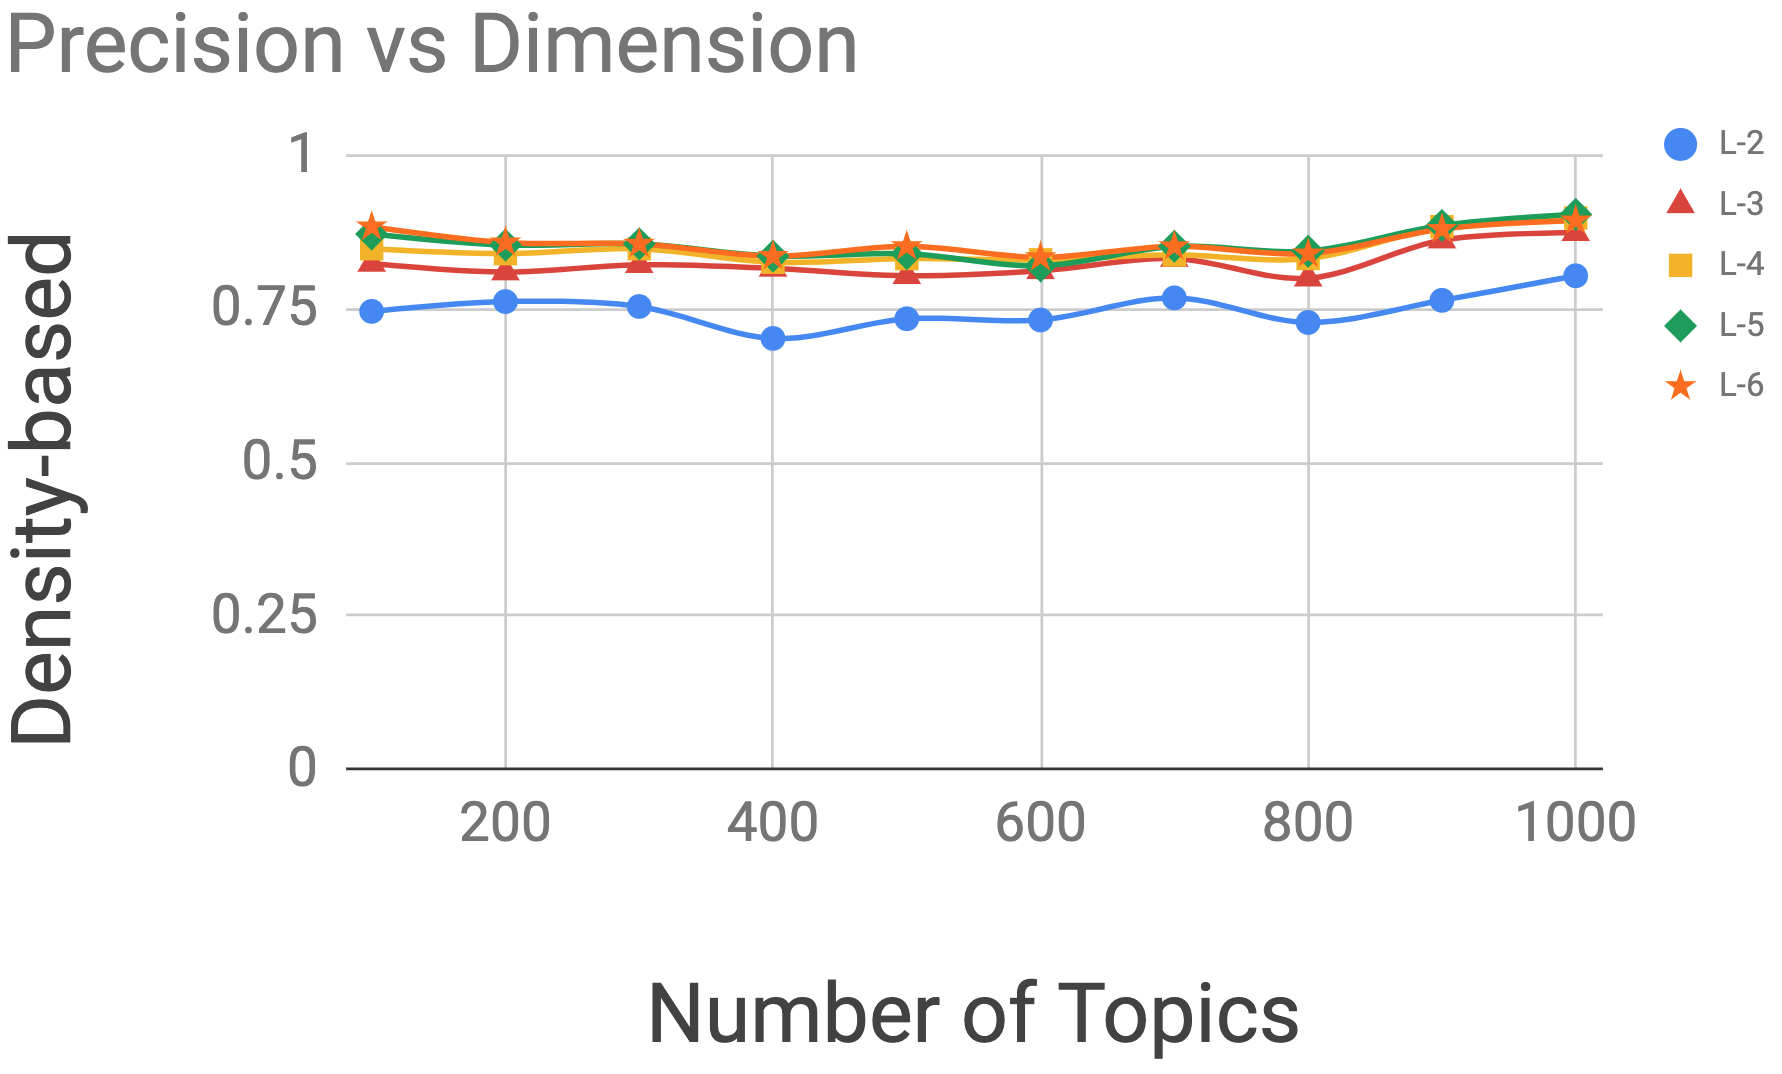
\includegraphics[scale=0.25]{dhhm-pd.png}
\caption{Precision at 5 (\textit{mean}) of threshold-based hashing method when number of topics varies in CORDIS dataset.}
\label{fig:thhm_pd}
\end{figure}

\begin{figure}[t]\centering
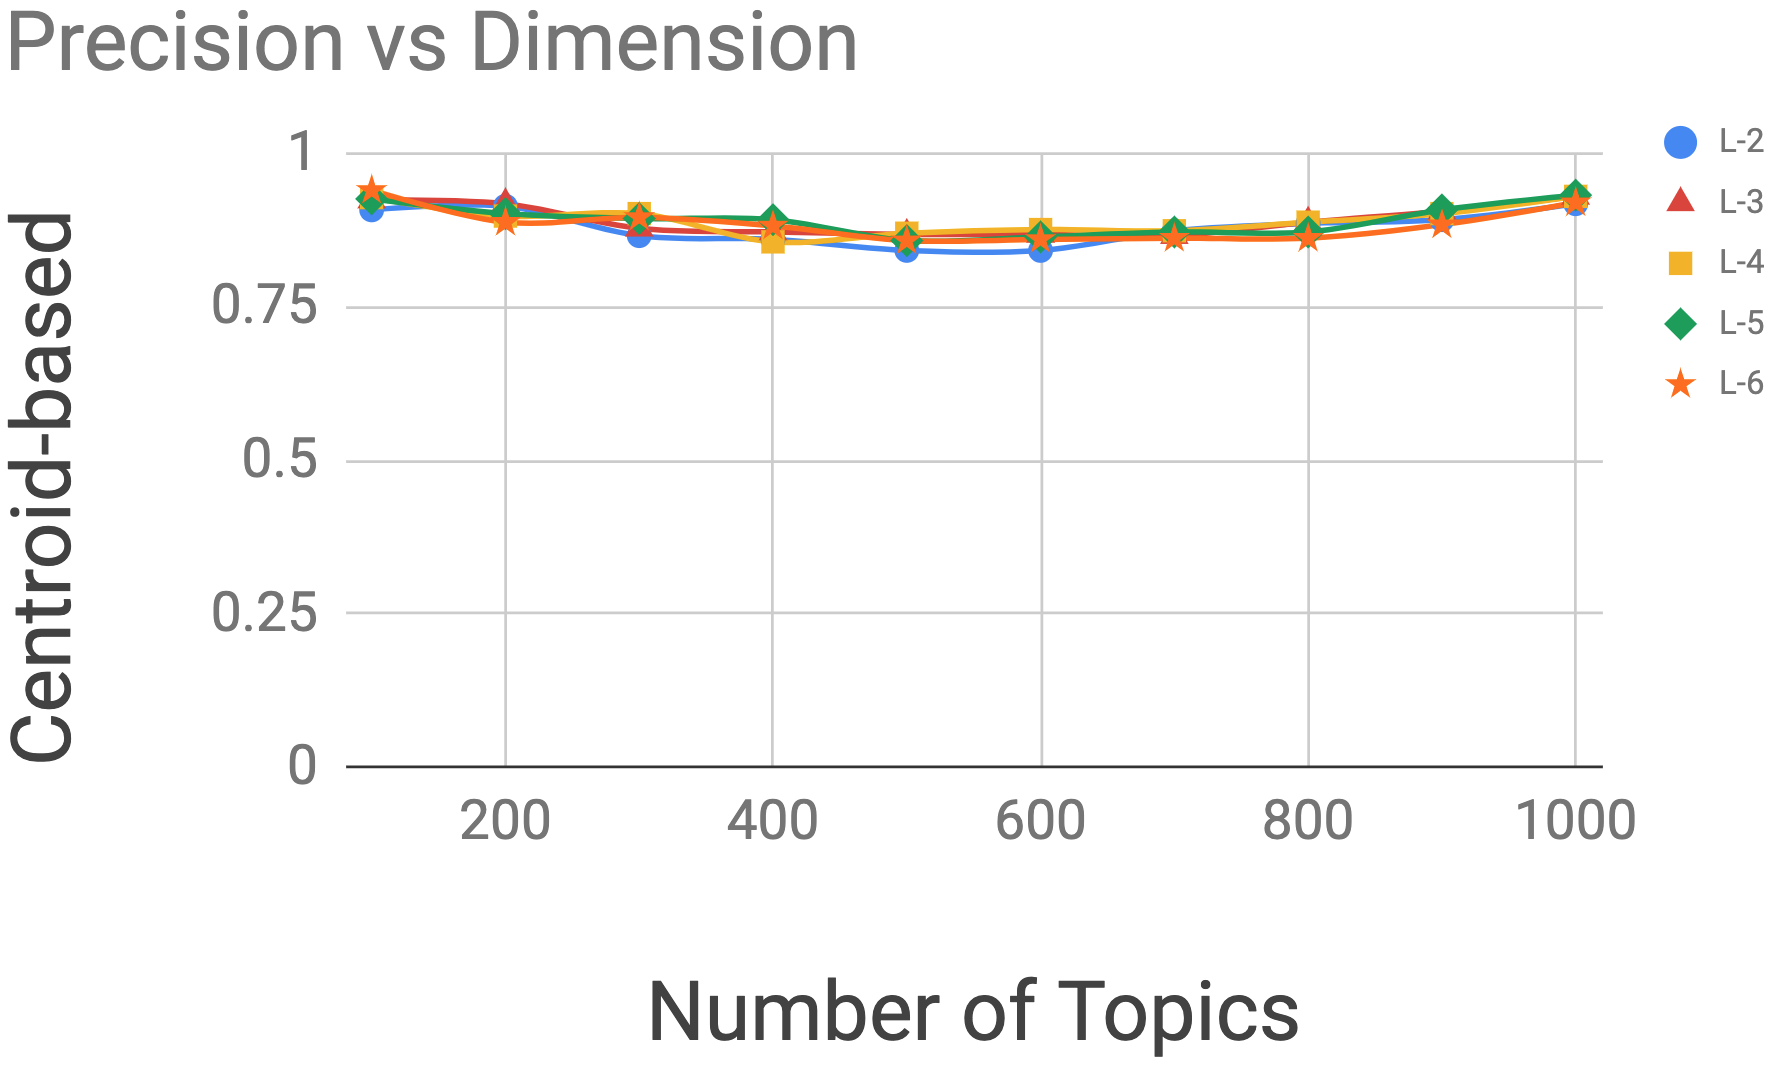
\includegraphics[scale=0.25]{chhm-pd.png}
\caption{Precision at 5 (\textit{mean}) of centroid-based hashing method when number of topics varies in CORDIS dataset.}
\label{fig:chhm_pd}
\end{figure}


\begin{figure}[t]\centering
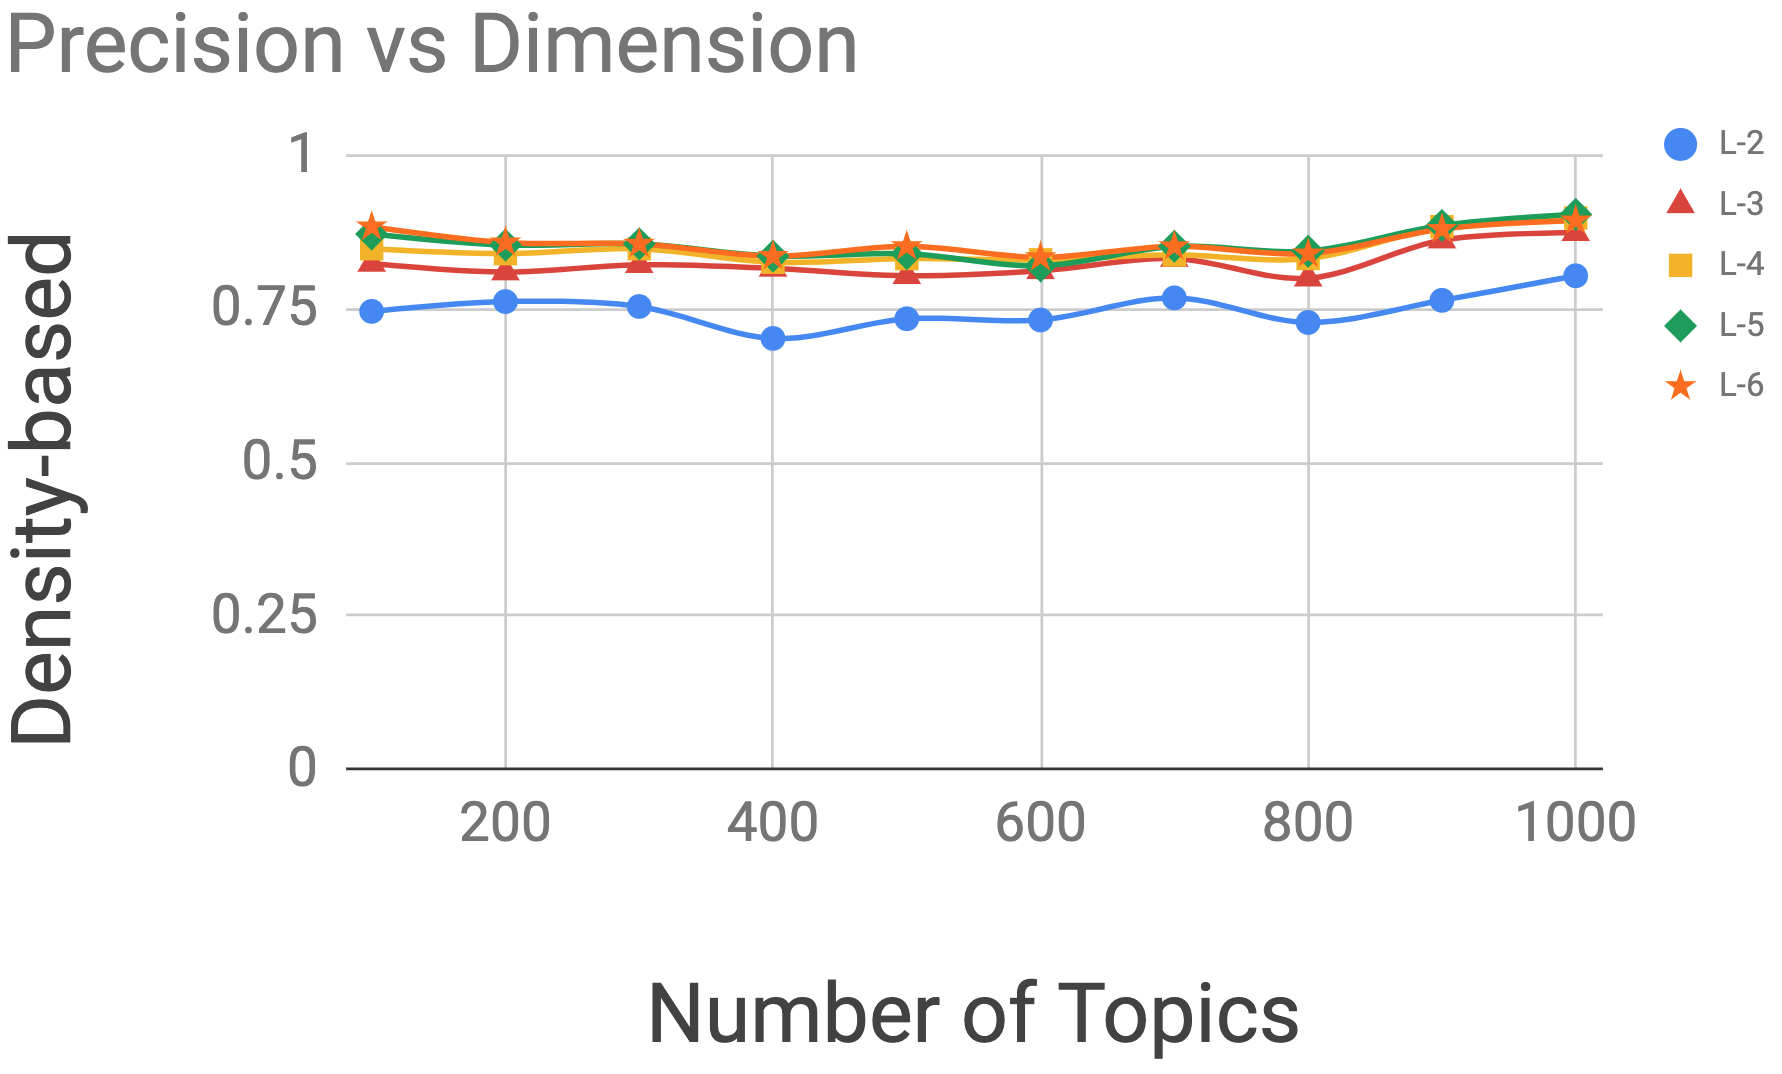
\includegraphics[scale=0.25]{dhhm-pd.png}
\caption{Precision at 5 (\textit{mean}) of density-based hashing method when number of topics varies in CORDIS dataset.}
\label{fig:dhhm_pd}
\end{figure}

Through the following example we describe the workflow to enable such retrieval operations. For simplicity we consider hash expressions with only two hierarchy levels. The reference document $d_1$ has the following hash expression: $h=\{h_0,h_1\}=\{(t10),(t18)\}$.

The first query, $Q1$, searches for documents similar to the reference document $d_1$ among all documents in the corpus. One of the ways to formalise this query looks like this: $Q1=h_0:t10$\^{}$100$ or $h_0:t18$\^{}$50$ or $h_1:t10$\^{}$50$ or $h_1:t18$\^{}$100$.  It sets a maximum boost (100) when the same restrictions as the reference document ($t10$ in $h_0$ and $t18$ in $h_1$) are fulfilled, and a lower boost (50) for the others ($t18$ in $h_0$ and $t10$ in $h_1$). In the specific case of applying this query to the CORDIS dataset, we observed that most of the retrieved documents included topic t18 (fig \ref{fig:exploration}).


But if we were only interested in similar documents to $d_1$ that have topic $t10$, we could restrict the previous query $Q1$ to express this condition in the following way: $Q2=(h_0:t10$\^{}$100$ or $h_1:t10$\^{}$50$) and ($h_1:t10$\^{}$50$ or $h_1:t18$\^{}$100$). The result obtained by $Q2$ (fig \ref{fig:exploration}) shows that the condition has been considered since there is a balance between topics $t10$ and $t18$ among the documents similar to $d_1$.

This type of restrictions based on the semantics offered by topics in the hash expression get enabled thanks to the methods proposed in this work.

\begin{table}\centering
\small
\begin{tabular}{ |c||c|c||c|  }
 \hline
 \multicolumn{4}{|c|}{OPEN-RESEARCH-100} \\
 \hline
 \textbf{hash} & \textbf{q1} & \textbf{q2} & \textbf{ratio} \\
 \hline
 thhm & 499,755 & 160,660 & 67.8 \\
 chhm & 356,111 & 1,976 & 99.44  \\
 dhhm & 49,068 & 766 & 98.43 \\
 \hline
\end{tabular}
\caption{Number of documents similar to a given one (q1) and also in a specific domain (q2) for threshold-based (thhm), centroid-based (chhm) and density-based (dhhm) hierarchical hashing methods.}
\label{tb:exploration}
\end{table}

\begin{figure}[t]\centering
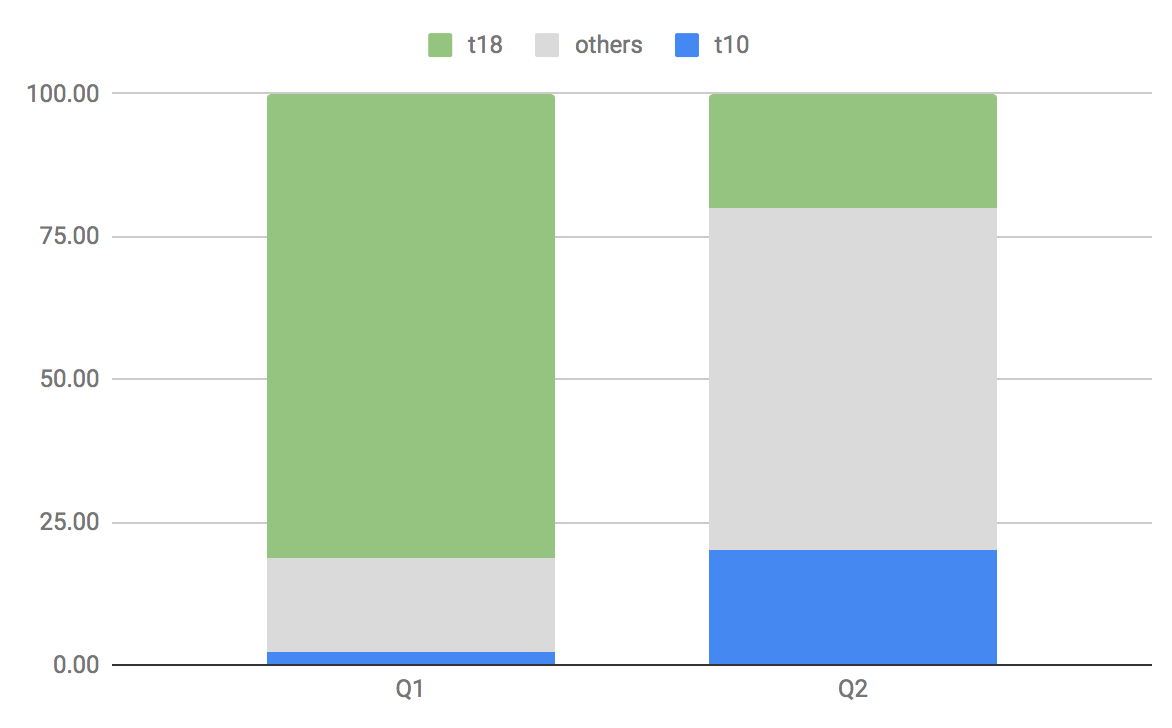
\includegraphics[scale=0.35]{exploration.png}
\caption{Most relevant topics in similar documents from using a document as query (Q1) and setting topic t10 as mandatory (Q2).}
\label{fig:exploration}
\end{figure}


\section{Summary}

The usefulness of topics created by probabilistic models when exploring document collections on large-scale has been widely studied in the literature. Each document in the corpus is described by probability distributions that measure the presence of those topics in their content. These vectors can also be used to measure the similarity between documents by using metrics such as Jensen-Shannon divergence (see Section \ref{sec:related-work}). But with large amounts of items in the collection, discovering the entire set of nearest neighbors to a given document would be infeasible. Due to the low storage cost and fast retrieval speed, hashing is one of the popular solutions for approximate nearest neighbors. However, existing hashing methods for probability distributions only focus on the efficiency of searches from a given document, without handling complex queries or offering hints about why one document is considered more similar than another. 

In this chapter we have introduced a new data structure to represent hash codes, based on topic  hierarchies created from the topic distributions. This approach has proven to obtain high-precision results and can accommodate additional query restriction. In doing so, we have showed a new way to annotate documents by topic inferences made from topic models. This addresses the technical objective of this thesis T03 (\textit{integrate the annotation method based on topic hierarchies into the topic model service}).

This way of encoding documents can also help to understand why two documents are similar, based on the intersection of topics at hierarchies of relevance. We have proposed a method to compare and organize huge document collections based on similar topic-based annotations, thus addressing the research objective R05 (\textit{define nearest-neighbor techniques to organize documents in regions with similar topic hierarchies}).

In addition, we have implemented the technique to compare documents in our librAIry framework, encouraging the achievement of the T04 technical objective (create a system capable of finding similar documents automatically).